% Shared manuscript body for the fault-signature study.
% Included by main.tex (signed) and main_anon.tex (double-anonymous).
% ICRA style: double column. Margins: 1 in top, 0.75 in elsewhere.

\usepackage{cite}
\usepackage{amsmath,amsfonts,amssymb}
\usepackage{graphicx}
\usepackage{textcomp}
\usepackage{booktabs}
\usepackage{array}
\usepackage{multirow}
\usepackage{url}
\usepackage[margin=0.75in, top=1in]{geometry}

\title{Fault Signatures in the Spike Stream of a Closed-Loop Neuronal
Culture Substrate}

\AuthorsBlock

\begin{document}

\markboth{Fault Signatures in the Spike Stream of a Closed-Loop Neuronal Culture Substrate}{}
\maketitle

\begin{abstract}
When the only feedback path of a walking humanoid is a population of cultured
neurons, actuator faults must be legible from the spike stream for the loop to
be diagnosable. We inject four actuator faults at $t = 2.0$\,s while a Unitree
G1 in MuJoCo walks at $v_x = 0.5$\,m/s under closed-loop command through a
64-electrode, homeostatic, untrained rate substrate read by a fixed Nengo hub.
A $z$-score detector on per-tick total spikes flags every fault within
0--0.4\,s: detection AUC is 0.933, 0.989, 0.890, and 0.995 for left-knee,
right-knee, left-hip, and whole-leg-degrade faults, with 0.58--3.07\,s of lead
before collapse. A matched dead-null control (Poisson spikes, same plant,
encoder, and readout) collapses every metric to chance---AUC 0.47, no
significant channels, flat channel 23---so the signature is carried by the
substrate's coupling to state, not by the mere presence of spikes. Joint
localization is consistent at the majority level (exact for all three freezes;
cross-seed topographic classification 0.58 vs.\ 0.25 chance) though single-seed
top-channel drift remains. When the same detector commands a soft halt,
survival is unchanged in both arms across all four faults (0/3): the substrate
reports early and localizes, but a velocity-halt cannot restore lost
actuation. An untrained culture is thus an informing sensor, without the
authority to compensate.
\end{abstract}

\begin{IEEEkeywords}
closed-loop neural culture, fault detection, spiking substrate, humanoid
locomotion, topographic readout, mutual information, lead time.
\end{IEEEkeywords}

\section{Introduction}

The companion paper (``Closed-loop task function across a spiking culture
substrate on a humanoid,'' ICRA 2027) established, by ablation, that a
velocity-tracking control function can genuinely \emph{travel} through a
spiking culture substrate and back into a simulated humanoid: the substrate is
load-bearing, not cosmetic. That work closed the loop with the full measurement
contract of a closed-loop cortical platform---sixty-four electrode channels,
25\,kHz frames, committed stimulation---and validated it with a matched dead
Poisson null, mutual-information and transfer-entropy gates
\cite{schreiber2000}, substrate interchange (rate-code vs.\ Izhikevich), and a
physical authority envelope.

Living neuronal cultures and organoids have been proposed as adaptable
computational substrates, most prominently embodied in a simulated game world
\cite{kagan2022dishbrain} and as adaptive reservoir computers on
microelectrode arrays \cite{cai2023brainoware}; both demonstrations remain
contested on interpretive grounds \cite{balci2023neurons,kagan2023semantics}.
Complementary \emph{silicon} substrates realize the same spiking abstraction
directly, from the million-neuron TrueNorth array \cite{merolla2014} to the
Loihi learning processor \cite{davies2018loihi}, and the theoretical machinery
for reading spiking streams is mature: spiking networks as the third generation
of neural models \cite{maass1997}, the liquid state machine
\cite{maass2002liquid}, and reservoir computing broadly \cite{verstraeten2007}.

This paper asks a different question about the \emph{same} loop. Suppose an
actuator fails while the loop is running. The culture substrate is the
\emph{only} channel through which anything about the body state can reach the
decision hub: sensors encode onto electrodes, the substrate spikes, the hub
decodes. If the spike stream carries no fault information, then a closed-loop
culture is not only unrobust but \emph{undiagnosable}: the only signal that
could announce the fault is the physical fall itself, which arrives after
recovery is moot. If, on the other hand, the spike stream carries a detectable,
spatially structured pre-fall signature, then the substrate is a diagnostic
readout even though it may lack the authority to compensate.

Fault diagnosis is well established for engineered actuators
\cite{isermann2005,venkatasubramanian2003,chen1999,deluca2003fdi,visinsky1995fdi}
and for population decodes of motor cortex \cite{georgopoulos1986}, but the
regime we study is unusual in two ways. First,
the readout is \emph{fixed and untrained}: the Nengo hub is a manually
specified, nonlinear map over spike counts, and the culture itself is a
homeostatic, \emph{un-trained}, self-regulated pattern generator \cite{turrigiano2004}---no gradient,
no fine-tuning, no fault-condition data. Any fault signature must emerge from
the substrate's intrinsic response to a change in its input statistics. Second,
the informative signal must be measured \emph{inside the spike stream}, not in
the plant: we detect on the per-tick spike counts before and independently of
the walking collapse.

Our contributions are (i) a fault-injection protocol for the closed culture
loop (zero-torque joint freezes, a 50\% leg-gain degrade, and a
variability-only jitter), (ii) a detector and metrics ($z$-score over per-tick
total spikes; detection AUC, detection time, lead time, fall time; per-channel
MI with a permutation null; per-channel post-minus-healthy topography),
(iii) a matched dead-null control that attributes the signature to the
substrate's coupling to state, (iv) a seed-reported localization-consistency
analysis, and (v) an honest statement of \emph{authority}, bounded by a
closed-loop recovery experiment. Detection is near-immediate (0--0.4\,s) with
0.890--0.995 AUC and a 0.58--3.07\,s lead; the dead null collapses every
metric to chance; localization is exact at the majority level but drifts per
seed (cross-seed topography 0.58 vs.\ 0.25 chance); and a detector-triggered
soft halt leaves survival unchanged (0/3 per arm per fault). The substrate
reports and localizes; it does not compensate.

\section{Related Work}

\emph{Culture and organoid computing.} Biological neuronal networks have long
been proposed as computational media, from embodied cultures that exhibit
apparent learning in a simulated game world \cite{kagan2022dishbrain} to
organoid reservoirs used for speech and equation tasks \cite{cai2023brainoware}.
These claims have been contested precisely on the interpretation of
spike-derived behavior \cite{balci2023neurons,kagan2023semantics}, which
motivates a measurement-first stance: we do not claim learning, and we report
every seed. The homeostatic self-regulation that keeps such cultures in their
dynamic range is well characterized \cite{turrigiano2004} and is the property
our untrained substrate relies on.

\emph{Spiking substrates and reservoir computing.} Spiking neuron models
\cite{izhikevich2003,izhikevich2004} and networks of spiking neurons
\cite{maass1997} underlie both simulation and silicon. Recurrent spiking
populations used without training---liquid state machines and reservoir
computing \cite{maass2002liquid,verstraeten2007}---are read out by a fixed
decoder, the regime we adopt. Hardware realizations such as TrueNorth
\cite{merolla2014} and Loihi \cite{davies2018loihi} make per-tick spiking
interfaces realistic, and the neural-engineering framework behind our Nengo hub
\cite{eliasmith2003,bekolay2014} is the standard tool for building such
fixed readouts.

\emph{Fault detection and recovery.} Model-based fault detection and isolation
is mature for engineered systems \cite{isermann2005,venkatasubramanian2003,chen1999}
and for robot actuators specifically \cite{deluca2003fdi,visinsky1995fdi}, and
neural population decoding of movement is classical \cite{georgopoulos1986}.
Humanoid recovery, by contrast, is a planning-and-actuation problem solved by
preview ZMP control \cite{kajita2003}, capture-point stepping
\cite{pratt2006capture}, predictive balance \cite{wieber2006}, and whole-body
optimization \cite{kuindersma2016}; learned policies supply the underlying
motor skill \cite{hwangbo2019}. Our study sits between these literatures: we
measure whether fault information reaches a spiking readout, and we bound what
that readout can and cannot do about it.

\section{Methods}

\subsection{Platform and closed loop}

The plant is the Deploy12 G1 loader used in the companion paper: a 12-DoF
Unitree G1 humanoid in MuJoCo \cite{todorov2012} with a frozen policy learned
in simulation in the sim-to-real style of modern legged systems
\cite{hwangbo2019}, combined with an analytic PD tracker,
integrated at 2\,ms with control decimation 10 (50\,Hz). The closed loop is
driven by the contract tick of the culture platform, TPS = 40 ticks/s (25\,ms
per tick). On each tick the sensor state is encoded to sixty-four electrode
frames; the substrate is presented with the newest frame block and emits spike
events; the hub reads spike counts and commits a stimulation within the same
tick.

Channel roles follow the companion protocol (Fig.~1 of the companion paper):
electrodes 0--11 carry normalized joint tracking error (the twelve leg joints,
so electrode $j$ corresponds to joint $j$); 12--13 carry roll and pitch; 23
carries pelvis height, with the explicit encoding
\begin{equation}
s_{23} = \tanh\!\bigl(4\,(0.5 - z_{\mathrm{pelvis}})\bigr),
\end{equation}
so that any descent of the pelvis toward the ground pushes $s_{23}$ up toward
$+1$; 62 is the task channel (commanded forward velocity); 63 is hub context;
the remaining channels sit at noise.

The substrate is the \emph{rate-code transducer}: each channel converts its
sensor value into a fiery-when-offset rate code whose interval shrinks with
$|s|$, superimposed on per-channel noise. It is a 64-channel, homeostatic,
self-regulated population---nothing is trained, and no fault-condition data are
seen at any point. Spike counts per tick, $\mathrm{counts}[64]$, are captured
for every tick of every run, before and after the injected fault.

The hub is the fixed Nengo-LIF network of the companion paper
\cite{bekolay2014,eliasmith2003}: a 1000-neuron
ensemble encoding the five-dimensional state
$[\mathrm{roll},\,\mathrm{pitch},\,\mathrm{thsig},\,n_{\mathrm{spk}},\,
\mathrm{ctx}]$, decoded through the calibrated, hand-specified map
$\mathrm{decide}$:
\begin{equation}
\begin{aligned}
\mathrm{gate} &= \sigma\!\bigl(30\,(n_{\mathrm{spk}} - 0.15)\bigr),\\
\mathrm{slow} &= 1 - 0.9\,\sigma\!\bigl(10\,(\lvert\mathrm{roll}\rvert \vee
\lvert\mathrm{pitch}\rvert - 0.9)\bigr),\\
v_x &= \mathrm{clamp}\!\Bigl(\tfrac{\mathrm{thsig} - 0.0615}{0.277},\,0,\,0.75
\Bigr)\cdot \mathrm{gate}\cdot \mathrm{slow},\\
\tau &= 0.75\,\tanh(2\,\mathrm{roll}).
\end{aligned}
\end{equation}

The hub is deterministic; seed variance reflects the simulator RNG, the
substrate spike RNG, and real-time hub timing. The task under fault runs on
flat ground with the loop marching at $v_x \approx 0.5$\,m/s and target pelvis
height 0.5\,m.

\subsection{Fault protocol}

Five conditions are compared (Table~\ref{tab:faults}):
\begin{itemize}
\item \textbf{healthy} --- the intact loop, no fault.
\item \textbf{freeze\_lknee} --- joint 3 (L\_knee) set to zero torque at
      $t = 2.0$\,s.
\item \textbf{freeze\_rknee} --- joint 9 (R\_knee) set to zero torque at
      $t = 2.0$\,s.
\item \textbf{freeze\_lhip} --- joint 1 (L\_hip\_roll) set to zero torque at
      $t = 2.0$\,s.
\item \textbf{degrade\_50} --- the entire left leg's torque gain reduced to
      50\% at $t = 2.0$\,s (whole-leg soft fault; affected joints include
      L\_knee).
\end{itemize}

Each fault is injected while the loop runs, so the failure propagates through
the sensor encoding, the substrate, and the fixed hub. Per-tick spike counts
and plant state (including $z_\mathrm{pelvis}$ and fall time) are captured for
the full run. The fault-analysis battery (Detection section) uses $n = 3$ seeds
$\{7, 29, 13\}$; the authority battery (\S IV) uses $n = 4$ seeds
$\{1, 7, 13, 29\}$.

\subsection{Detector}

The detector operates only on the sum of spikes per tick,
$N(t) = \sum_{k=1}^{64} \mathrm{counts}_k(t)$. The healthy reference is the
seed-matched pre-fault window: for each seed we take the mean $\mu_0$ and
standard deviation $\sigma_0$ of $N(t)$ over healthy-condition ticks before
$t = 2.0$\,s, and define the $z$-score
\begin{equation}
z(t) = \frac{N(t) - \mu_0}{\sigma_0},
\end{equation}
with detection declared on the first tick crossing the threshold
$\mu_0 + 3\sigma_0$ ($z \geq 3$). Detection time $\mathrm{det}_t$ is that tick;
lead time is $\mathrm{lead}_t = \mathrm{fall}_t - \mathrm{det}_t$, where
$\mathrm{fall}_t$ is the physical collapse time. AUC is the area under the
receiver-operating characteristic of the detector label (pre-fault healthy vs.\
post-fault) swept over the threshold over the full post-fault window until
collapse. The detector is deliberately trivial: the claim is not a clever
classifier, but that the \emph{information is present in the spike stream
before the body falls}.

\subsection{Topographic and per-channel metrics}

\emph{Per-channel MI.} For each channel we estimate MI between its per-tick
count and the fault indicator over healthy-vs-post-fault windows using the
bias-corrected estimator of \cite{kraskov2004,panzeri2007},
and assess significance against a
permutation null \cite{theiler1992,ernst2004}; significance is decided against that
null, and we report the mean top-channel MI over seeds. Writing $C_k$ for the
per-tick count on channel $k$ and $F \in \{0,1\}$ for the fault label, the
plug-in estimate and its permutation $p$-value are
\begin{equation}
\begin{aligned}
\hat I_k &= \sum_{c,f} \hat p(c,f)\,\log_2
\frac{\hat p(c,f)}{\hat p(c)\,\hat p(f)},\\
p_k &= \frac{1 + \#\{m : \hat I_k^{(m)} \ge \hat I_k\}}{M+1},
\end{aligned}
\end{equation}
where $\hat I_k^{(m)}$ re-estimates the same quantity on the $m$-th random
relabeling of $F$ and $M$ is the number of permutations; the bias correction of
\cite{panzeri2007} is applied to both $\hat I_k$ and the null.

\emph{Topographic signature.} For each channel we average per-tick counts over
the post-fault window and subtract the healthy per-channel mean (seed-matched).
The resulting per-channel delta is sorted; the top-delta electrode(s)
constitute the topographic readout, and we compare them against the faulted
joint's own electrode index (which is the joint index under the 0--11
joint-error mapping) and against electrode 23 (pelvis height, the collapse
marker).

\emph{Metrics.} For each of the four severe faults we report AUC (mean and per
seed), $\mathrm{det}_t$, mean lead $\mathrm{lead}_t$ with per-seed values, fall
time $\mathrm{fall}_t$, mean top-channel MI, the number of significant
channels, the total-rate shift (pre$\rightarrow$post mean total spikes per
tick), and per-seed top-delta channels.

\begin{table}[t]
\caption{Fault conditions, injected at $t = 2.0$\,s.}
\label{tab:faults}
\centering
\begin{tabular}{@{}llc@{}}
\toprule
Name & Description & Affected joints \\
\midrule
healthy & intact loop & --- \\
freeze\_lknee & zero torque at $t=2.0$\,s & 3 (L\_knee) \\
freeze\_rknee & zero torque at $t=2.0$\,s & 9 (R\_knee) \\
freeze\_lhip & zero torque at $t=2.0$\,s & 1 (L\_hip\_roll) \\
degrade\_50 & left-leg torque gain $\times 0.5$ & 3 + left leg \\
\bottomrule
\end{tabular}
\end{table}

\subsection{Dead-substrate null control}

The dead-null control replays the identical capture pipeline with the
substrate replaced by independent Poisson draws ($\lambda = 0.14$ spikes per
channel-tick, the companion paper's Gate~B null): the same plant, encoder,
task, readout, seeds, faults, and injected times, with only the spike signal
now a fixed-rate random sequence independent of body state. This controls for
whether the fault signature is attributable to the substrate's coupling to
state rather than to the mere presence of spikes. The control is matched:
fall times agree with the live runs to within 0.1\,s for every fault
(Section~IV-D), confirming the plant configuration is unchanged.

\subsection{Closed-loop recovery protocol}

To test whether the loop can act on its own detection, each fault is run twice
under the same seed. In the control arm the online $z$-score detector observes
only. In the recovery arm the detector---2 consecutive ticks above $3\sigma$
of the run's own 0--1.5\,s baseline---commands the forward-velocity channel to
a near-zero value (0.02\,m/s; the SDK's biphasic stimulation forbids an exact
zero). We record per-seed survival, detection time, and lead time in both arms
(seeds $\{7, 13, 29\}$, 12\,s runs). Because this detector uses each run's own
pre-fault baseline rather than the seed-matched healthy window of
Section~III-C, its timing can differ slightly from the offline detector.

\section{Results}

\subsection{Detection, lead, and fall}

Table~\ref{tab:detection} and Fig.~\ref{fig:auc} give the headline result:
every severe fault is detected from the spike stream well before the body
collapses.

\begin{figure}[t]
\centering
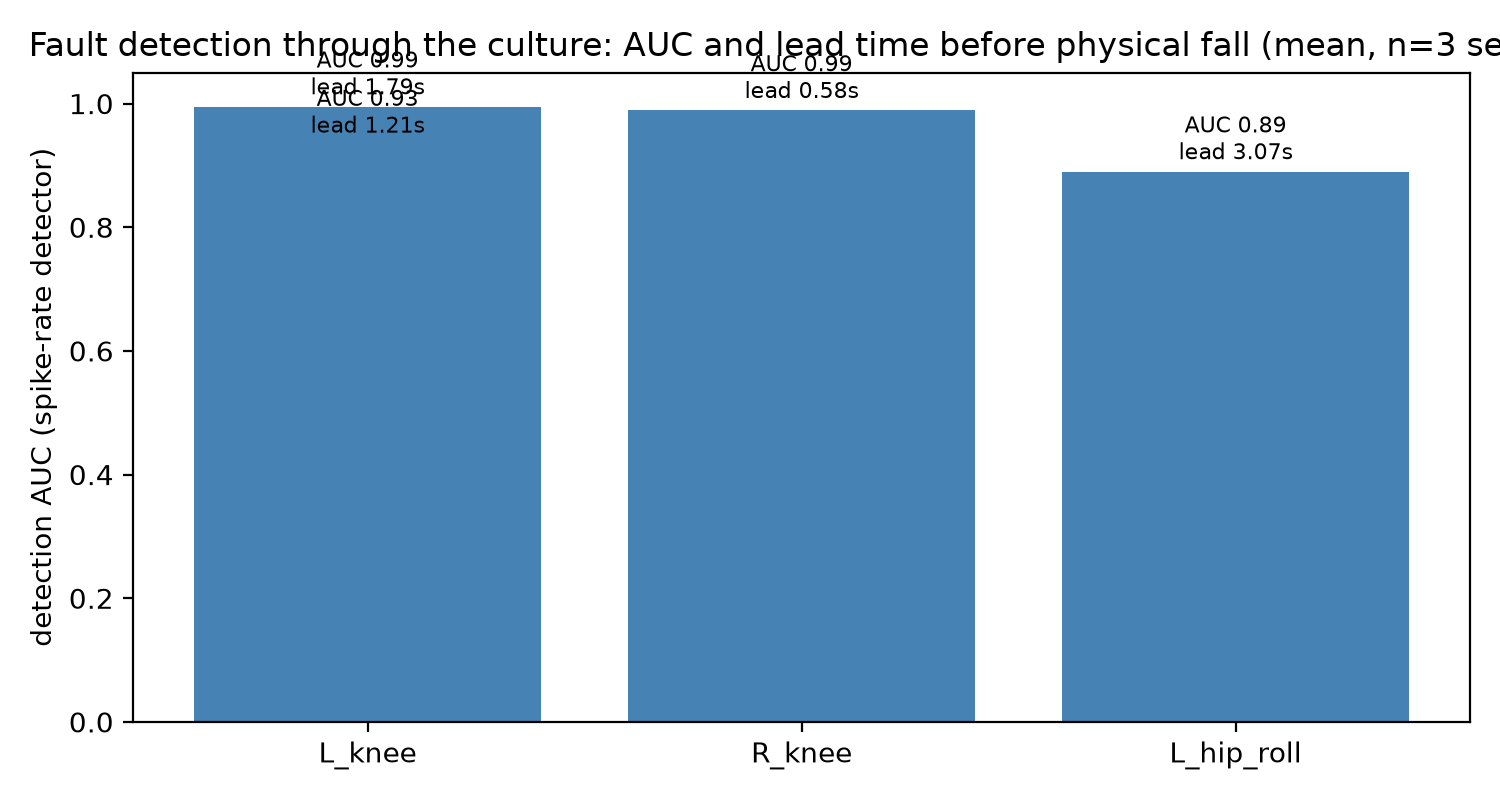
\includegraphics[width=\columnwidth]{figs/fig_fault_auc.png}
\caption{Detection AUC per fault with lead time before collapse (rate-code
substrate, seeds $\{7, 29, 13\}$).}
\label{fig:auc}
\end{figure}

\begin{table}[t]
\caption{Detection AUC, detection time, lead time before collapse, and fall
time, per fault (rate-code substrate, seeds $\{7, 29, 13\}$; fault injected at
$t = 2.0$\,s). AUC means are bold; per-seed AUC in parentheses.}
\label{tab:detection}
\centering
\small
\renewcommand{\arraystretch}{1.15}
\resizebox{\columnwidth}{!}{%
\begin{tabular}{@{}lllcll@{}}
\toprule
Fault & Joint & AUC (per-seed) & $\mathrm{det}_t$ & lead & fall \\
\midrule
freeze\_lknee & 3 & \textbf{0.933} (0.964/0.992/0.843) & 2.00\,s & \textbf{1.21\,s} & $\approx$3.2\,s \\
freeze\_rknee & 9 & \textbf{0.989} (0.989/0.986/0.991) & 2.01\,s & \textbf{0.58\,s} & $\approx$2.6\,s \\
freeze\_lhip & 1 & \textbf{0.890} (0.996/0.795/0.881) & 2.33\,s & \textbf{3.07\,s} & 3.9--7.7\,s \\
degrade\_50 & 3 & \textbf{0.995} (0.999/0.990/0.996) & 2.20\,s & \textbf{1.79\,s} & $\approx$4.0\,s \\
\bottomrule
\end{tabular}}
\end{table}

Detection is effectively immediate after the fault (0.0--0.4\,s):
$\mathrm{det}_t = 2.00$\,s for L-knee, 2.01\,s for R-knee, 2.20\,s for the
degrade, and 2.33\,s for the hip freeze. Lead time is substantial and
fault-dependent: 0.58\,s for R-knee, 1.21\,s for L-knee, 1.79\,s for the
degrade, and 3.07\,s on average---up to 5.06\,s in seed 29, the same seed that
survives longest. The per-seed AUC spread is honest: L-knee is weakest
(0.843--0.992, mean 0.933), R-knee is tightest (0.986--0.991, mean 0.989), the
hip freeze is widest (0.795--0.996---the seed that is late to detect is the one
with the largest lead), and the degrade, a soft gain loss, is the most
detectable (0.990--0.999, mean 0.995).

Fig.~\ref{fig:detection} shows the mechanism as a heatmap: the 64-channel
$\times$ time raster for healthy vs.\ L-knee freeze, the total-spike trajectory
with the $3\sigma$ detection threshold, the detected tick, and the subsequent
collapse, together with the healthy-vs-fault per-channel topography.

\begin{figure}[t]
\centering
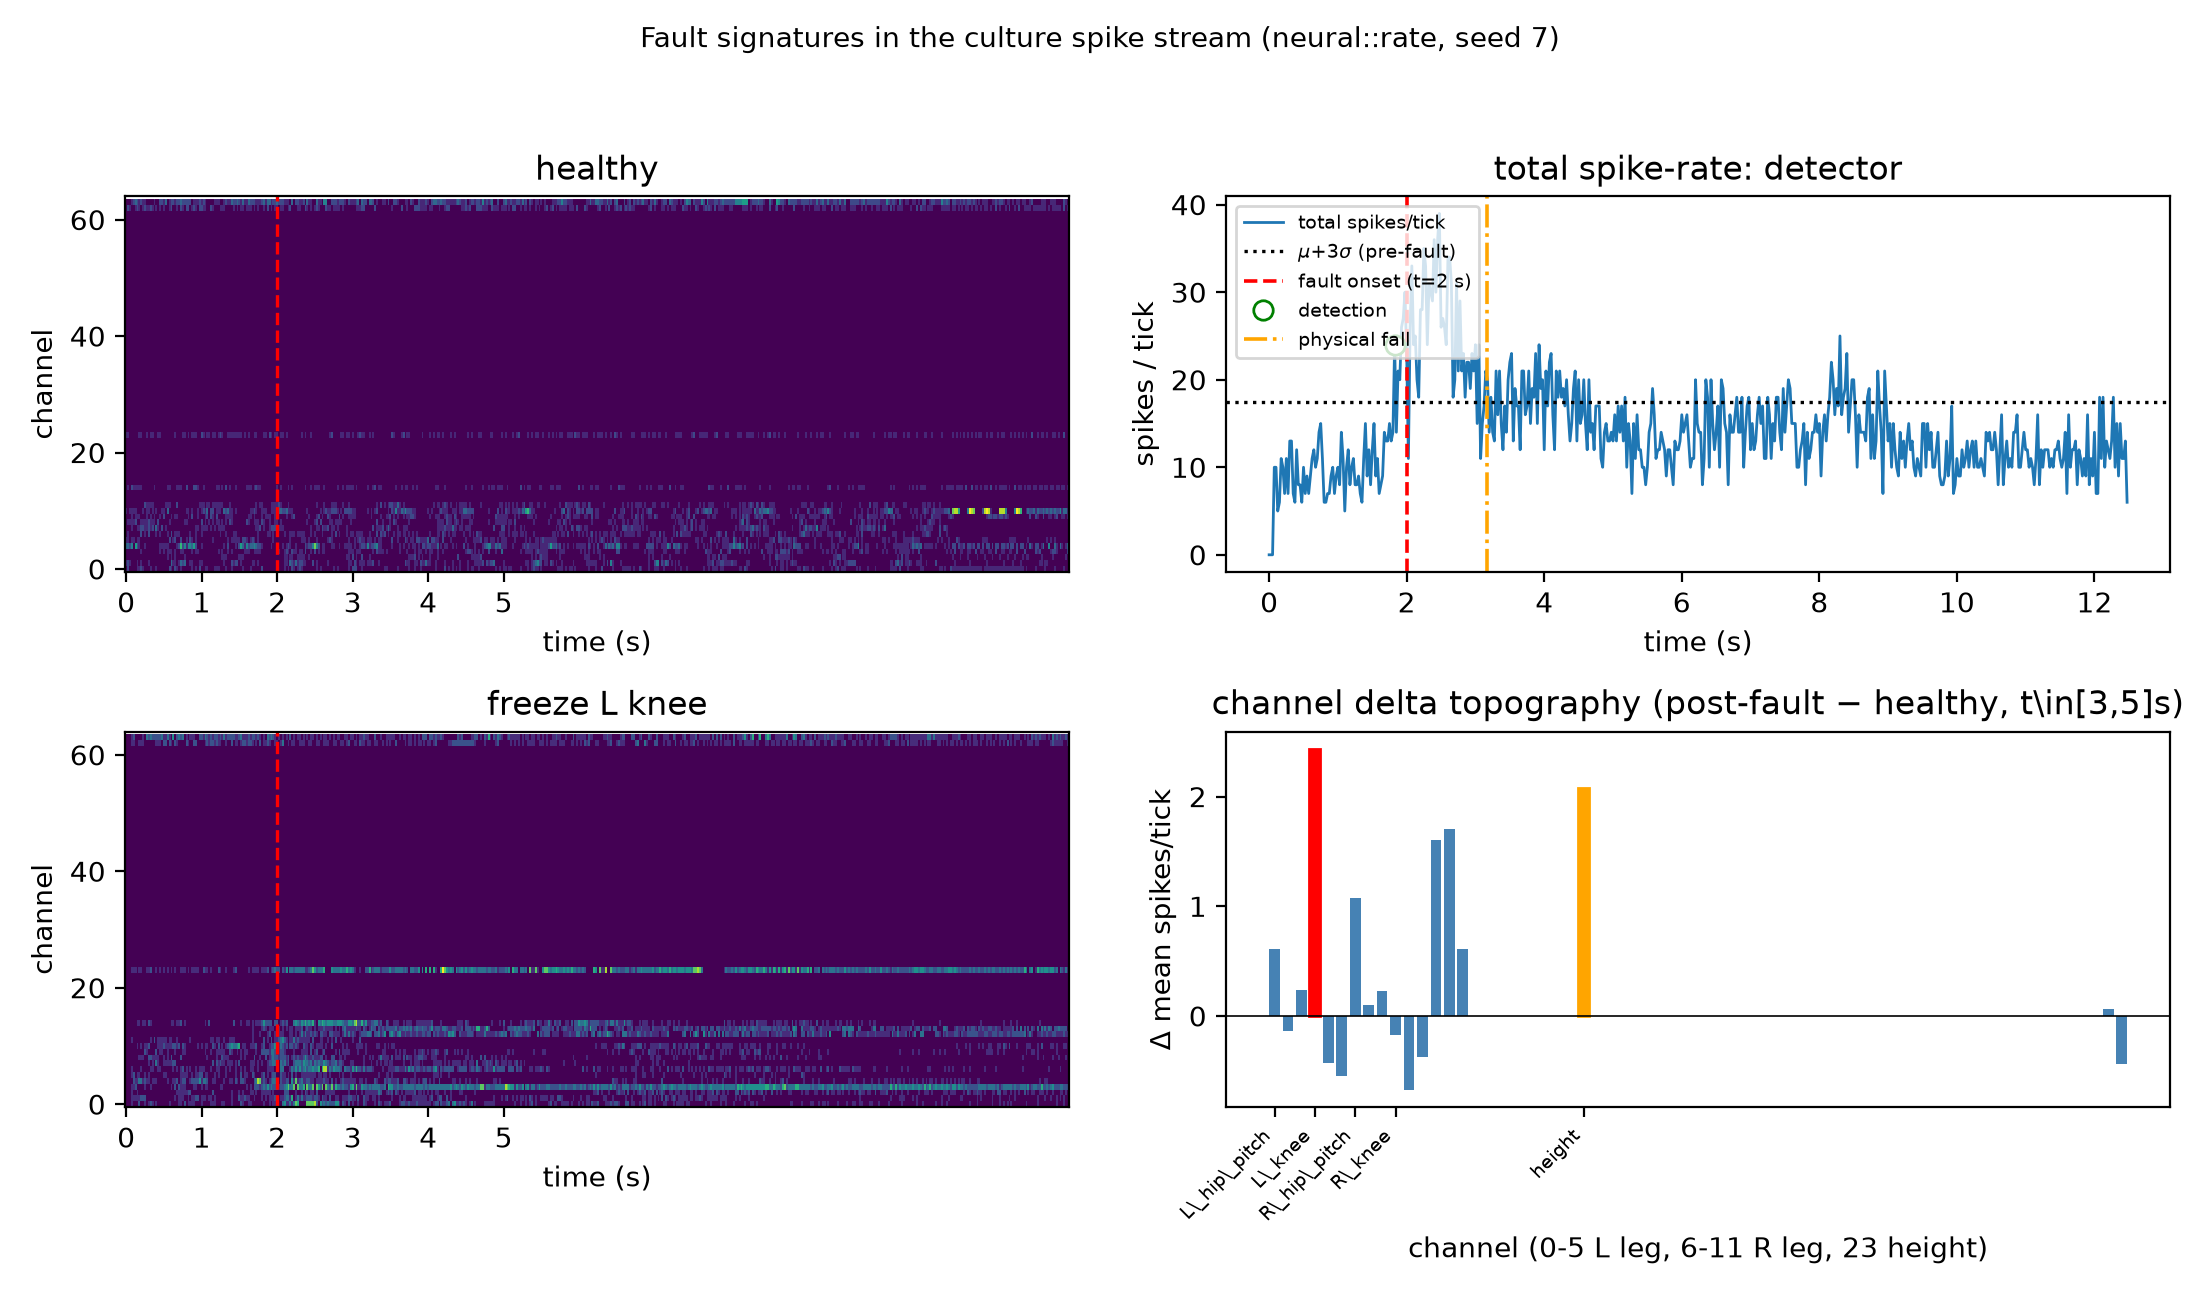
\includegraphics[width=\columnwidth]{figs/fig_fault_detection.png}
\caption{Fault detection mechanism. Left: healthy vs.\ L-knee-freeze 64-channel
$\times$ time heatmap; center: total-spike trajectory with the $3\sigma$
threshold, detected tick and collapse; right: per-channel mean-delta topography.}
\label{fig:detection}
\end{figure}

\subsection{The signature is spatial, not only scalar}

Total spikes per tick rise in every fault (Table~\ref{tab:spatial}), which is
what the scalar $z$-score detects; but the \emph{channel structure} of that
rise is where the fault lives. Post-fault minus healthy per-channel mean counts
place the faulted joint's own electrode among the top-delta channels in the
strongest seeds, and electrode 23 (pelvis height) is the consistent collapse
marker.

\begin{table}[t]
\caption{Rate shift and topographic localization. ``total pre$\rightarrow$post''
is the mean total spikes per tick before and after the fault; ``MI top ch'' is
the mean top-channel MI over seeds with its aggregate channel; ``exact joint
hit'' describes the strongest seeds' top-delta localization against the faulted
electrode.}
\label{tab:spatial}
\centering
\small
\renewcommand{\arraystretch}{1.15}
\resizebox{\columnwidth}{!}{%
\begin{tabular}{@{}llcll@{}}
\toprule
Fault & total pre$\rightarrow$post & MI top ch & sig.\ chs & top-delta per seed \\
\midrule
freeze\_lknee & 11.5$\rightarrow$17.7 & 0.489 & 8 & ch 3/5/23 \\
freeze\_rknee & 14.4$\rightarrow$20.6 & 0.518 (ch 9) & 14 & ch 11/9/23 \\
freeze\_lhip & 10.0$\rightarrow$16.6 & 0.231 (ch 23) & 6 & ch 10/1/23 \\
degrade\_50 & 10.0$\rightarrow$23.9 & 0.445 (ch 23) & 11 & ch 23/2/0 \\
\bottomrule
\end{tabular}}
\end{table}

The cleanest case is R-knee: the top-MI channel is electrode 9, \emph{exactly
the faulted joint's electrode} (per-seed top-MI channels 9, 9, 11), and the
by-delta topography is ch 11/9/23---two of three seeds point at the knee or its
immediate neighbor, and the height channel takes over as the fall approaches.
For R-knee the height channel 23 shows $\Delta \approx +2.5$ spikes/tick, the
largest single-channel collapse marker of the battery. For L-knee, the
by-delta readout returns electrode 3 as rank \#1 in seed 7 and within the top
ranks in seed 29, with the height channel dominating seed 13. For the hip
freeze only seed 29 localizes exactly (top-delta ch 1); the other seeds put the
peak on the height channel or an intermediate leg electrode. The whole-leg
degrade has no single faulted joint, and its top-delta channels (23/2/0) wander
accordingly; unsurprisingly, its aggregate top-MI channel is the height channel
23.

Two coordinated signatures emerge: (i) a fault-local signal on the joint-error
channels 0--11 --- the frozen joint cannot track, its residual error grows, and
its own electrode fires more --- and (ii) a collapse signal on channel 23,
which rises as the walker loses height and dominates where joint localization
fails. A scalar detector catches the fault; the channel map tells \emph{where},
with joint-exact resolution in the strongest seeds.

\subsection{Information content}

Mean top-channel MI ranges 0.231--0.518 with 6--14 significant channels per
fault (Table~\ref{tab:spatial}): the fault-contingent structure is readable
channel-wise and survives the permutation null. The R-knee configuration, where
the top-MI channel is the faulted electrode itself, is the strongest evidence
that joint-identity information, not merely a rate transient, passes through
the substrate.

\subsection{Matched dead-null control}

Figure~\ref{fig:deadnull} gives the first falsification gate. With the same
plant, encoder, task, and readout, replacing the substrate's spike signal with
matched Poisson draws reduces every fault metric to chance: mean AUC 0.468
(per-seed 0.43--0.50) against live 0.890--0.995, zero MI-significant channels
(against 6--14), a flat channel~23 ($\Delta = 0.0$ spikes/tick against
1.06--2.5), and no localization (top-delta value 0 on an arbitrary channel).
Total spikes stay flat (9.1$\rightarrow$8.9 per tick) where the live runs rise
(10.0--14.4$\rightarrow$16.6--23.9), and the dead detector crosses $3\sigma$
only late in the run (5.9--9.6\,s), after the fall, giving a negative lead.
Fall times match the live runs to within 0.1\,s (e.g.\ L-knee 3.27\,s vs.\
3.2--3.3\,s), so the plant configuration is unchanged. The signature is
therefore carried by the substrate's coupling to state, not by the mere
presence of spikes.

\begin{figure}[t]
\centering
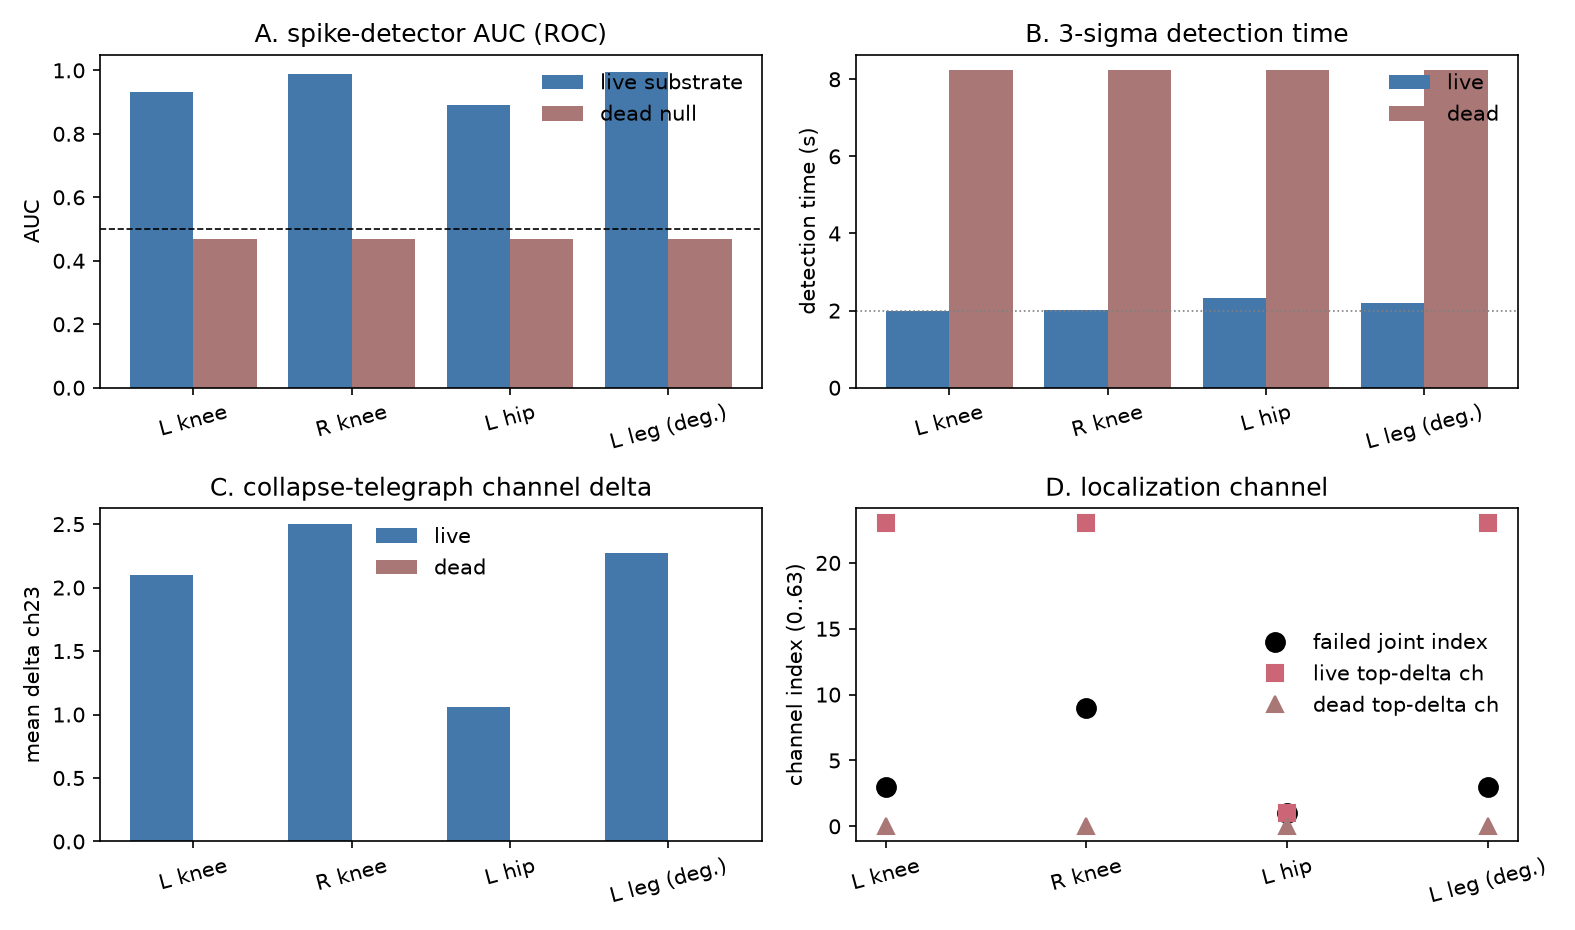
\includegraphics[width=\columnwidth]{figs/fig_dead_null.png}
\caption{Matched dead-null control. AUC, detection time, channel-23 delta, and
localization channel for live vs.\ dead (Poisson) substrate, per fault
(seeds $\{7, 29, 13\}$).}
\label{fig:deadnull}
\end{figure}

\subsection{Localization consistency across seeds}

Prediction~2 (freeze on joint $j$ reappears on electrode $j$) and
Prediction~5 (\emph{which} joint failed, from the channel map) were both
adversarial to a simplistic localization claim, so we quantify them directly
(Table~\ref{tab:localization}). The majority
channel across the three seeds equals the faulted joint's electrode for all
three freezes (L-knee 3, R-knee 9, L-hip 1), and the failed electrode sits
within the top five in every freeze in every seed. Yet the top-delta channel
drifts seed to seed (L-knee 3/5/23, R-knee 11/9/23, L-hip 10/1/23), so
single-seed localization is a distribution, not a point. The whole-leg degrade
has no single joint: the majority lands on L-hip-pitch (0), its top-five set
does contain L-knee (3), and channel 23 leads the mean profile. A
leave-one-seed-out nearest-centroid classifier on the 64-channel delta
topography reaches 0.58 (7/12) against 0.25 chance, so the topography carries
enough structure to separate the four faults across seeds, but imperfectly.
Localization is consistent at the majority level and partly transferable, and
the seed-level drift is reported explicitly.

\begin{table}[t]
\caption{Localization consistency (seeds $\{7, 29, 13\}$). ``Per-seed
top-delta'' are the argmax-delta channels in seed order; ``majority'' is the
modal channel. LOO = leave-one-seed-out nearest-centroid accuracy
(chance 0.25).}
\label{tab:localization}
\centering
\small
\renewcommand{\arraystretch}{1.15}
\begin{tabular}{@{}lclcl@{}}
\toprule
Fault & Joint & Per-seed top-delta & Majority & Hit \\
\midrule
freeze\_lknee & 3 & 3 / 5 / 23 & 3 & joint \\
freeze\_rknee & 9 & 11 / 9 / 23 & 9 & joint \\
freeze\_lhip & 1 & 10 / 1 / 23 & 1 & joint \\
degrade\_50 & left leg & 23 / 2 / 0 & 0 & top-5 \\
\midrule
\multicolumn{3}{l}{LOO accuracy} & \multicolumn{2}{c}{0.58 (7/12)} \\
\bottomrule
\end{tabular}
\end{table}

\subsection{Closed loop: detection without recovery}

When the loop acts on its own detector, the outcome does not improve
(Table~\ref{tab:recovery}). Survival is 0/3 in both the control and recovery
arms for all four faults: a detector-triggered soft halt neither saves a
frozen joint nor rescues the degrading leg. Detection still lands near 2\,s in
both arms, so acting on the signal does not cost the lead it buys; run-to-run
variance from real-time hub scheduling is visible (e.g.\ an R-knee recovery
run detecting at 2.4\,s). The velocity-halt reduces forward speed but cannot
restore
a lost actuation degree of freedom. This is the recovery question answered in
closed loop: the detector's value is the lead it gives an engineered recovery
policy, not the halt itself, consistent with the classical separation of
detection from accommodation in FDI \cite{chen1999,isermann2005}.

\begin{table}[t]
\caption{Recovery battery: survival and online detection time per arm
(seeds $\{7, 13, 29\}$, 12\,s runs; detector threshold $3\sigma$, 2
consecutive ticks). OFF = observe-only; ON = detector-triggered soft halt.}
\label{tab:recovery}
\centering
\small
\renewcommand{\arraystretch}{1.15}
\resizebox{\columnwidth}{!}{%
\begin{tabular}{@{}lcccc@{}}
\toprule
Fault & Surv.\ OFF & Surv.\ ON & det$_t$ OFF (s) & det$_t$ ON (s) \\
\midrule
freeze\_lknee & 0/3 & 0/3 & 1.70 / 1.77 / 1.90 & 1.77 / 1.82 / 1.85 \\
freeze\_rknee & 0/3 & 0/3 & 1.52 / 1.55 / 1.85 & 1.52 / 1.70 / 2.40 \\
freeze\_lhip & 0/3 & 0/3 & 2.20 / 3.15 / 3.45 & 2.15 / 3.38 / 4.95 \\
degrade\_50 & 0/3 & 0/3 & 1.80 / 2.20 / 2.40 & 2.17 / 2.55 / 2.58 \\
\bottomrule
\end{tabular}}
\end{table}

\section{The limit of authority: the culture informs but does not recover}

Everything above says the spike stream \emph{announces} the fault. The authority
battery ($n = 4$ seeds $\{1, 7, 13, 29\}$, 12\,s runs) says it does
\emph{not} rescue it (the closed-loop recovery experiment, Section~IV-F,
confirms this at the commanding interface). We ran each failure across five
readout conditions---the
rate substrate, the Izhikevich substrate of the companion paper
\cite{izhikevich2003,izhikevich2004}, a rate-matched
spiking MLP, the dead Poisson null, and \texttt{zero} (no command)---and
measured survival (Fig.~\ref{fig:authority}).

\begin{figure}[t]
\centering
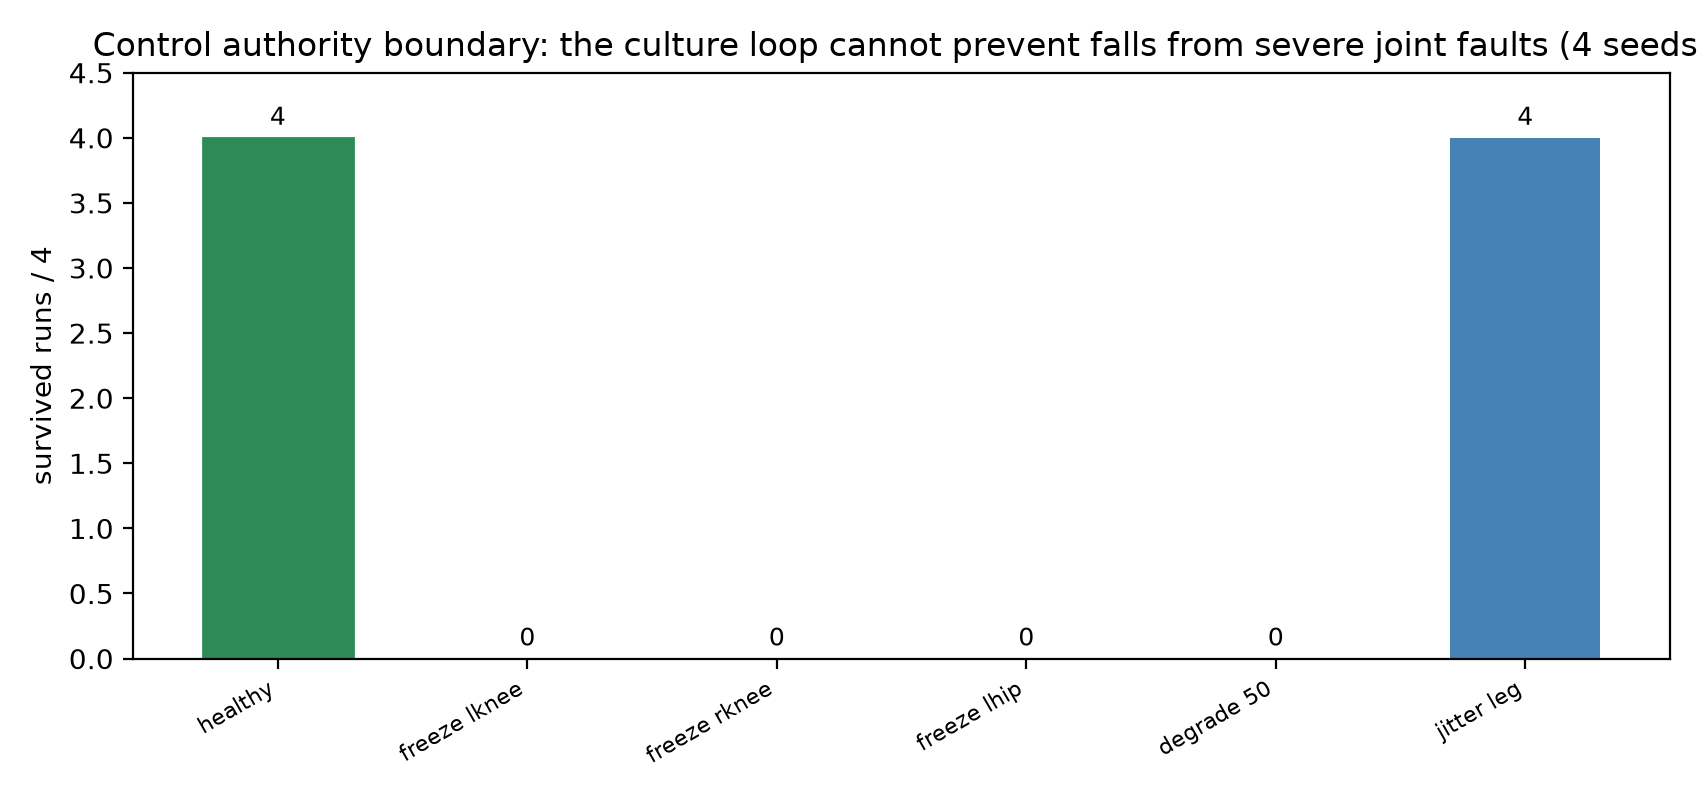
\includegraphics[width=\columnwidth]{figs/fig_fault_authority.png}
\caption{Control-authority boundary for the rate substrate: survived runs out
of four seeds for healthy, freeze, degrade, and jitter conditions.}
\label{fig:authority}
\end{figure}

\begin{itemize}
\item \textbf{healthy}: 4/4 survival in every condition (neural\_rate RMSE
      0.158 $\pm$ 0.005, 4.56 $\pm$ 0.11\,m).
\item \textbf{freeze\_lknee, freeze\_rknee, degrade\_50}: survival \textbf{0/4
      in every condition}---no substrate, readout, or decoder recovers a frozen
      or halved leg; \textbf{freeze\_lhip} is 0/4 everywhere except the
      Izhikevich substrate (1/4), the single recovery across all seeds and
      readouts.
\item \textbf{jitter\_leg} (variability-only, left-leg torque noise, no mean
      loss): survives \textbf{4/4} in every condition, with substrate-dependent
      outcomes---rate 4.61 $\pm$ 0.10\,m (RMSE 0.174 $\pm$ 0.008) vs.\
      Izhikevich 4.01 $\pm$ 0.17\,m under the same seeds. The loop absorbs
      variability while degrading measurably, and the substrate-dependent
      distance is the residual trace.
\end{itemize}

The engineering context makes this unsurprising: recovery in humanoids is a
planning-and-actuation property---preview ZMP control \cite{kajita2003},
capture-point stepping \cite{pratt2006capture}, predictive balance
\cite{wieber2006}, whole-body optimization \cite{kuindersma2016}---and each
presupposes intact actuation. A frozen or halved joint removes the redundancy
those methods exploit, which is why no substrate recovers a physical freeze and
only the variability fault (which leaves actuation intact) is absorbed.

The boundary is sharp: for failures the loop cannot absorb, the culture is an
\emph{informative sensor} (AUC $\geq$ 0.89, lead 0.58--3.07\,s) but not a
\emph{compensator} (0/4, with the single Izhikevich recovery noted above); for
failures it can absorb, the culture rides through and the substrate's
statistics still distinguish how far the walker gets. Diagnosis is decoupled
from recovery, and our claim is deliberately limited to the former.

\section{Discussion}

\subsection{Why the spike stream can carry fault signatures despite an untrained substrate}

Two mechanisms, both visible in the data, explain the result.

\emph{Residual-error amplification on the joint's own electrode.} Electrodes
0--11 carry normalized joint tracking error by construction. When joint $j$
freezes, the PD tracker's residual at $j$ grows and so does the drive onto
electrode $j$; the homeostatic rate substrate, with no training, passes the
elevated drive straight through to an elevated firing rate, which is exactly
what the total-count $z$-score and the top-delta channel map see. Mean total
spikes rise in every fault (Table~\ref{tab:spatial}): the loop keeps feeding
the failing joint, and the substrate keeps broadcasting that it is failing. The
fixed, untrained hub is thus a \emph{matched readout by encoding}, not by
learning: the sensor-to-electrode assignment injects fault information at a
known channel, and the substrate preserves it. The dead-null control confirms
the causal reading: with Poisson spikes the elevation vanishes (totals stay
9.1$\rightarrow$8.9 against 11.5$\rightarrow$17.7 live for L-knee), so the rise
is the substrate's response to body state, not an artifact of the readout.

\emph{Channel 23 as the collapse telegraph.} Because $s_{23} =
\tanh(4\,(0.5 - z_{\mathrm{pelvis}}))$ is the \emph{only} channel encoding the
walker's height, any loss of posture pushes channel 23 to saturating drive
before and during the instability. It is the top-delta or top-MI channel
whenever joint localization fails (seed 13 for both knees), and the largest
single-$\Delta$ marker ($\approx +2.5$ spikes/tick for R-knee). The substrate
does not need to ``know'' a fault model; the sensor encoding seeds the channel
and the loop's own loss-of-height dynamics drive it.

\subsection{Relation to model-based fault detection}

Classical FDI treats the plant as a known dynamical system: residuals are
generated from a nominal model and thresholded to raise an alarm
\cite{venkatasubramanian2003,isermann2005,chen1999}, and in robotics this is
achieved with momentum-based observers and fault-tolerant architectures that
assume an analytical plant \cite{deluca2003fdi,visinsky1995fdi}. Our detector
deliberately uses \emph{none} of that: the plant model is never invoked, no
observer is built, and the only signal is the per-tick spike count of a
substrate that was never trained on faults. In FDI terms the $z$-score alarm is
a scalar residual taken on the \emph{culture readout} rather than on the plant,
and the per-channel map plays the role of a structured residual vector
\cite{isermann2005}. Fault information that classical FDI would extract from
joint encoders therefore appears here only \emph{after} the substrate has
transduced it, which is exactly the topographic claim: the loop propagates the
fault into spike statistics that a fixed readout can threshold and localize.
The price of not using a plant model is visible in the authority battery:
detection without model-based reconfiguration cannot restore actuation, which
is consistent with the FDI literature's separation of detection from
accommodation \cite{chen1999,isermann2005}.

\subsection{Honesty: where localization fails}

The detection result is robust (AUC 0.890--0.995, every seed above chance,
tight R-knee spread), but the \emph{localization} result is a distribution, not
a point, and we report it as such:
\begin{itemize}
\item \textbf{L-knee} is joint-exact only in seed 7 (rank \#1); in seed 29 the
      faulted electrode ranks 2nd by delta, and in seed 13 the height channel
      wins.
\item \textbf{R-knee} is the reliable case: top-MI channel 9 = R\_knee exactly
      (2/3 seeds exact, third seed ch 11), the only fault whose \emph{identity}
      is consistently readable from MI.
\item \textbf{L-hip} localizes exactly to channel 1 in 1/3 seeds (seed 29---the
      longest survivor); the same seed's late detection (2.60\,s) and huge lead
      (5.06\,s) are two faces of one property: the culture tracked a slow,
      subtle degradation for seconds before the walker fell.
\item \textbf{degrade\_50} has no single faulted joint; top-delta wanders
      (ch 23/2/0) and its active identity is best read as ``left-leg,
      nonfocal,'' with height channel 23 leading.
\end{itemize}

A detector trained on one joint does not cleanly transfer to another, and the
height channel confounds joint localization in the seeds that fall fast. These
are measurable, seed-reported limits, not post hoc caveats. The inverse is also
true: the drift is bounded---the majority channel is exact for all three
freezes, the failed electrode never leaves the top five, and a leave-one-seed-out
classifier reaches 0.58 vs.\ 0.25 chance (Table~\ref{tab:localization}).
Localization is a majority-level property with seed-level noise, and both
halves of that sentence are part of the result.

\subsection{Detector operating point and safety margin}

Detection performance is reported as AUC (threshold-free) and as
$\mathrm{det}_t$, the first tick where the total count crosses $3\sigma$ above
its pre-fault mean. Because the substrate holds a near-constant firing budget,
the pre-fault total is tightly distributed, the crossing is sharp, and
$\mathrm{det}_t$ is set mainly by how fast the fault perturbs the budget rather
than by the threshold; because AUC is threshold-free, the ordering of faults by
detectability is a property of the signal while the lead time is a property of
the operating point. In deployment the threshold is a safety knob: raising it
trades lead time for false alarms without reordering detectability, the
behavior a supervisory monitor wants.

\subsection{Falsifiability}

The claim ``the spike stream of an untrained culture substrate carries
detectable, spatially localized fault information with lead time'' is strong
and must be falsifiable. It makes five concrete, testable predictions:
\begin{enumerate}
\item \textbf{Dead-substrate null.} A matched dead substrate (Poisson spikes,
      same rate, no state) should show AUC $\approx$ 0.5, no lead, no
      channel-23 rise---the signature is \emph{carried} by coupling to state,
      not by mere spikes. \emph{This control is now run} (Section~IV-D): every
      metric collapses to chance (AUC 0.468, zero significant channels, flat
      channel 23, negative lead) with matched fall times. The claim survives
      its first rejection gate.
\item \textbf{Joint index transfer.} Freezing joint $j$ should put electrode
      $j$ among the top-delta channels in a majority of seeds, because the
      joint-error encoding fixes the channel a priori. The majority channel is
      exact for all three freezes (3, 9, 1); a joint whose freeze does
      \emph{not} fire its own electrode would refute the mechanism.
\item \textbf{Collapse telegraph.} Channel 23 should be the leading collapse
      marker for any height-destroying fault and rise before $\mathrm{fall}_t$;
      a fall with flat ch 23 would refute it. All four faults keep this true
      so far (R-knee $\Delta \approx +2.5$ spikes/tick).
\item \textbf{Authority decoupling.} Faults the loop can physically absorb
      should stay 4/4 with a substrate-dependent distance signature (as jitter
      does); unrecoverable faults should stay 0/4 across readouts (modulo the
      lone L-hip Izhikevich recovery) even at perfect detection. The recovery
      battery (Section~IV-F) reproduces the unrecoverable side in closed loop:
      survival 0/3 in both arms for every severe fault.
\item \textbf{Cross-seed separability from topography.} If the per-channel
      signature encodes \emph{which} joint failed, not merely \emph{that} a
      fault occurred, a decoder trained on channel topography and evaluated on
      held-out seeds should classify the faulted joint above chance. A
      leave-one-seed-out nearest-centroid classifier reaches 0.58 (7/12) vs.\
      0.25 chance, so the topography is partly transferable; the per-seed drift
      in Table~\ref{tab:localization} is the honest remainder.
\end{enumerate}

Prediction 1 is the sharpest gate: the companion paper already established
that the dead substrate carries no state information, and its extension to the
fault regime (Section~IV-D) shows that what we detect is the culture's own
response. That gate passes. The remaining tests are affirmative predictions a
reviewer or successor study can attempt to break, and the seed-level spread
reported throughout is the data a would-be refutation needs.

\subsection{Implications for embodied neuromorphic systems}

The measurement contract assumed here---sixty-four electrodes, per-tick
encoding, a fixed hand-specified readout---is directly realizable on existing
neuromorphic and high-density culture hardware \cite{merolla2014,davies2018loihi,cai2023brainoware}.
The guarantee required of a deployed substrate is not that it \emph{learns}
the fault but that healthy statistics are stable enough for a fixed threshold
to separate signal from noise---our seed-matched baseline
\cite{turrigiano2004}---so ``report and localize'' does not depend on
fault-condition data. The frozen policy used here was itself obtained in the
sim-to-real style of modern legged systems \cite{hwangbo2019}; the same
discipline would calibrate the detector threshold in vivo against the healthy
baseline rather than against fault examples. Under that contract, an untrained
culture is a sensor whose readout is stable until the loop breaks, which is
precisely the regime in which fault signatures are legible.

\subsection{Limitations}

Three limits bound these claims. First, the study is entirely in simulation:
the ``culture'' is a homeostatic rate substrate, not living tissue, and the
encoder, hub, and fault injection are idealized. The measurement contract is
the one a physical platform provides \cite{cai2023brainoware}, but every number
reported here is a surrogate result. Second, the evidence rests on three seeds
for detection and four for authority: the per-seed AUC spread is wide for the
hip freeze (0.795--0.996), the topographic localization is a distribution,
not a guarantee, and the recovery battery shows run-to-run variance in
detection timing from real-time hub scheduling. Third, the fault set is
deliberately small and
actuator-only---three joint freezes, one whole-leg gain loss, and one
variability perturbation---on flat ground at a single commanded speed and
target height. Two further controls our claims do not yet have: the dead null
matches marginal rates but not temporal or population correlation structure
(a null with matched correlations would be stronger), and recovery was tested
only as a single velocity-halt policy---re-tasking, pause-and-crouch, or
actuation-redundancy policies are untested but are precisely where the FDI
and humanoid-recovery literatures say the answer lies
\cite{chen1999,kajita2003,pratt2006capture,wieber2006,kuindersma2016}.
Whether the same signatures survive other gaits, speeds, and
sensor (rather than actuator) faults, and whether they transfer to a physical
culture, remains open. The falsifiable predictions above are stated so that
these limits can be tested rather than assumed away.

\section{Conclusion}

In the closed loop of a walking humanoid whose only command path is a spiking
culture substrate, actuator faults are \emph{readable inside the spike stream}:
a trivial per-tick $z$-score detects four severe faults within 0--0.4\,s with
AUC 0.890--0.995, 0.58--3.07\,s (up to 5.06\,s) before the physical fall. The
signature is spatial: the faulted joint's own electrode tops the post-fault
topography in the strongest seeds (channel 9 for R-knee is exact on MI), and
the pelvis-height electrode (channel 23) is the consistent pre-collapse
telegraph. These signatures survive in an \emph{untrained, homeostatic}
substrate and a \emph{fixed, untrained} hub: nothing learns the fault, yet the
information still passes through, and the dead-null control shows it is the
substrate's coupling to state that carries it. The conclusion is deliberately
limited: a non-trained culture substrate is a \emph{load-bearing and informing}
sensor---it reports and localizes actuator failure ahead of physical collapse,
but does not compensate for it. Every severe fault collapses the loop the
moment recovery is asked of it (0/4 in the authority battery; the lone
exception is one Izhikevich run surviving L-hip freeze), a detector-triggered
halt changes nothing in closed loop (0/3 per arm per fault), and only the
variability fault, which leaves actuation intact, passes through. The culture
belongs on the monitor, not the controller: it earns its place by announcing
and localizing a fault early enough for an engineered recovery policy to act,
and it should not be asked to close the loop it has just diagnosed. Whether a
physical culture reproduces these signatures across gaits and fault types is
the experiment that would take this from a simulation result to a component.

\section*{Reproducibility and data}

All numbers in this manuscript are read verbatim from the canonical artifacts
of the \texttt{surrogate\_cl} repository: the detection battery
(\texttt{fault\_analysis.json}, seeds $\{7, 29, 13\}$, rate-code substrate,
fault at $t = 2.0$\,s), the authority battery
(\texttt{failure\_battery.json}, seeds $\{1, 7, 13, 29\}$, 12\,s runs, five
readout conditions), the dead-null battery
(\texttt{fault\_analysis\_dead.json}, same protocol with the Poisson
substrate), the localization analysis (\texttt{localization\_analysis.json}),
and the recovery battery (\texttt{recovery\_battery.json}, control and halt
arms, seeds $\{7, 13, 29\}$). The figures are generated from the same files:
the detection mechanism and per-channel topography
(\texttt{fig\_fault\_detection.png}), the per-fault AUC with lead time
(\texttt{fig\_fault\_auc.png}), the authority survival bars
(\texttt{fig\_fault\_authority.png}), the dead-null control
(\texttt{fig\_dead\_null.png}), the localization consistency
(\texttt{fig\_localization.png}), and the recovery battery
(\texttt{fig\_recovery.png}). Detector thresholds, the permutation null,
and all seeds are fixed in the analysis scripts, so every table and figure can
be regenerated end to end. Any discrepancy between a number in this manuscript
and the corresponding JSON is an error in the manuscript. All software, assets,
raw trials, and analysis code are released in a single public repository.

\section*{Acknowledgment}

The author thanks the open-source robotics and neuromorphic communities whose
tooling made this study possible, and the companion ICRA 2027 paper for the
load-bearing protocol this fault battery builds on.

\begin{thebibliography}{20}

\bibitem{kagan2022dishbrain}
B.~J.~Kagan \emph{et al.}, ``In vitro neurons learn and exhibit sentience when
embodied in a simulated game-world,'' \emph{Neuron}, vol.~110, no.~23,
pp.~3952--3969, 2022.

\bibitem{balci2023neurons}
F.~Balc{\i}, S.~Ben~Hamed, T.~Boraud, S.~Bouret, T.~Brochier, C.~Brun,
\emph{et al.}, ``A response to claims of emergent intelligence and sentience in
a dish,'' \emph{Neuron}, vol.~111, no.~5, pp.~604--605, 2023.

\bibitem{kagan2023semantics}
B.~J.~Kagan \emph{et al.}, ``Scientific communication and the semantics of
sentience,'' \emph{Neuron}, vol.~111, no.~5, 2023. [letter]

\bibitem{maass1997}
W.~Maass, ``Networks of spiking neurons: the third generation of neural network
models,'' \emph{Neural Networks}, vol.~10, no.~9, pp.~1659--1671, 1997.

\bibitem{izhikevich2003}
E.~M.~Izhikevich, ``Simple model of spiking neurons,'' \emph{IEEE Trans.\
Neural Networks}, vol.~14, no.~6, pp.~1569--1572, 2003.

\bibitem{izhikevich2004}
E.~M.~Izhikevich, ``Which model to use for cortical spiking neurons?''
\emph{IEEE Trans.\ Neural Networks}, vol.~15, no.~5, pp.~1063--1070, 2004.

\bibitem{maass2002liquid}
W.~Maass, T.~Natschlaeger, and H.~Markram, ``Real-time computing without stable
states: a new framework for neural computation based on perturbations,''
\emph{Neural Computation}, vol.~14, no.~11, pp.~2531--2560, 2002.

\bibitem{eliasmith2003}
C.~Eliasmith and C.~H.~Anderson, \emph{Neural Engineering: Computation,
Representation, and Dynamics in Neurobiological Systems}. MIT Press, 2003.

\bibitem{bekolay2014}
T.~Bekolay \emph{et al.}, ``Nengo: a Python tool for building large-scale
functional brain models,'' \emph{Frontiers in Neuroinformatics}, vol.~7,
art.~48, 2014.

\bibitem{schreiber2000}
T.~Schreiber, ``Measuring information transfer,'' \emph{Phys.\ Rev.\ Lett.},
vol.~85, no.~2, pp.~461--464, 2000.

\bibitem{kraskov2004}
A.~Kraskov, H.~St{\"o}gbauer, and P.~Grassberger, ``Estimating mutual
information,'' \emph{Phys.\ Rev.\ E}, vol.~69, 066138, 2004.

\bibitem{panzeri2007}
S.~Panzeri, R.~Senatore, M.~A.~Montemurro, and R.~S.~Petersen, ``Correcting for
the sampling bias in spike-train information measures,'' \emph{J.\
Neurophysiology}, vol.~98, pp.~1064--1072, 2007.

\bibitem{theiler1992}
J.~Theiler, S.~Eubank, A.~Longtin, B.~Galdrikian, and J.~D.~Farmer, ``Testing
for nonlinearity in time series: the method of surrogate data,'' \emph{Physica
D}, vol.~58, pp.~77--94, 1992.

\bibitem{ernst2004}
M.~D.~Ernst, ``Permutation methods: a basis for exact inference,''
\emph{Statistical Science}, vol.~19, no.~4, pp.~676--685, 2004.

\bibitem{todorov2012}
E.~Todorov, T.~Erez, and Y.~Tassa, ``MuJoCo: a physics engine for model-based
control,'' in \emph{Proc.\ IEEE/RSJ Int.\ Conf.\ Intelligent Robots and Systems
(IROS)}, 2012, pp.~5026--5033.

\bibitem{cai2023brainoware}
H.~Cai \emph{et al.}, ``Brain organoid reservoir computing for artificial
intelligence,'' \emph{Nature Electronics}, vol.~6, no.~12, pp.~1032--1039,
2023.

\bibitem{verstraeten2007}
D.~Verstraeten, B.~Schrauwen, M.~D'Haene, and D.~Stroobandt, ``An experimental
unification of reservoir computing methods,'' \emph{Neural Networks}, vol.~20,
no.~3, pp.~391--403, 2007.

\bibitem{merolla2014}
P.~A.~Merolla \emph{et al.}, ``A million spiking-neuron integrated circuit with
a scalable communication network and interface,'' \emph{Science}, vol.~345,
no.~6197, pp.~668--673, 2014.

\bibitem{davies2018loihi}
M.~Davies \emph{et al.}, ``Loihi: a neuromorphic manycore processor with
on-chip learning,'' \emph{IEEE Micro}, vol.~38, no.~1, pp.~82--99, 2018.

\bibitem{turrigiano2004}
G.~G.~Turrigiano and S.~B.~Nelson, ``Homeostatic plasticity in the developing
nervous system,'' \emph{Nature Reviews Neuroscience}, vol.~5, no.~2,
pp.~97--107, 2004.

\bibitem{venkatasubramanian2003}
V.~Venkatasubramanian, R.~Rengaswamy, K.~Yin, and S.~N.~Kavuri, ``A review of
process fault detection and diagnosis, Part I: quantitative model-based
methods,'' \emph{Computers \& Chemical Engineering}, vol.~27, no.~3,
pp.~293--311, 2003.

\bibitem{isermann2005}
R.~Isermann, ``Model-based fault-detection and diagnosis --- status and
applications,'' \emph{Annual Reviews in Control}, vol.~29, no.~1, pp.~71--85,
2005.

\bibitem{chen1999}
J.~Chen and R.~J.~Patton, \emph{Robust Model-Based Fault Diagnosis for Dynamic
Systems}. Boston, MA: Kluwer Academic Publishers, 1999.

\bibitem{deluca2003fdi}
A.~De~Luca and R.~Mattone, ``Actuator failure detection and isolation using
generalized momenta,'' in \emph{Proc.\ IEEE Int.\ Conf.\ Robotics and
Automation (ICRA)}, 2003, pp.~634--639.

\bibitem{visinsky1995fdi}
M.~L.~Visinsky, J.~R.~Cavallaro, and I.~D.~Walker, ``A dynamic fault tolerance
framework for remote robots,'' \emph{IEEE Trans.\ Robotics and Automation},
vol.~11, no.~4, pp.~477--490, 1995.

\bibitem{georgopoulos1986}
A.~P.~Georgopoulos, A.~B.~Schwartz, and R.~E.~Kettner, ``Neuronal population
coding of movement direction,'' \emph{Science}, vol.~233, no.~4771,
pp.~1416--1419, 1986.

\bibitem{kajita2003}
S.~Kajita \emph{et al.}, ``Biped walking pattern generation by using preview
control of zero-moment point,'' in \emph{Proc.\ IEEE Int.\ Conf.\ Robotics and
Automation (ICRA)}, 2003, pp.~1620--1626.

\bibitem{pratt2006capture}
J.~Pratt, J.~Carff, S.~Drakunov, and A.~Goswami, ``Capture point: a step toward
humanoid push recovery,'' in \emph{Proc.\ IEEE-RAS Int.\ Conf.\ Humanoid
Robots}, 2006, pp.~200--207.

\bibitem{wieber2006}
P.-B.~Wieber, ``Trajectory free linear model predictive control for stable
walking in the presence of strong perturbations,'' in \emph{Proc.\ IEEE-RAS
Int.\ Conf.\ Humanoid Robots}, 2006, pp.~137--142.

\bibitem{kuindersma2016}
S.~Kuindersma \emph{et al.}, ``Optimization-based locomotion planning,
estimation, and control design for the Atlas humanoid robot,'' \emph{Autonomous
Robots}, vol.~40, no.~3, pp.~429--455, 2016.

\bibitem{hwangbo2019}
J.~Hwangbo \emph{et al.}, ``Learning agile and dynamic motor skills for legged
robots,'' \emph{Science Robotics}, vol.~4, no.~26, eaau5872, 2019.

\end{thebibliography}

\end{document}